\section{Avancement}

\subsection{Bibliothèques testées}

\subsubsection{Reconstruction 3D}

La reconstruction 3D étant un domaine de recherche répandu, un grand nombre d'algorithmes existe déjà. J'ai donc tenté de trouver une librairie permettant de reconstruire un nuage de points à partir d'une liste d'images.
On peut trouver plusieurs algorithmes sur OpenSLAM.org :
\begin{itemize}
  \item ScaViSLAM
  \item RobotVision
\end{itemize}

Cependant les travaux présents sur OpenSLAM.org sont généralement conçus pour des capteurs de type laser.

Il faut également que je regarde ce que propose la librairie MRPT\footnote{Mobile Robot Programming Toolkit}.

\subsubsection{Fusion de cartes}

Afin de fusionner des cartes j'ai testé l'algorithme ICP sur deux nuages de points ayant un nombre de points plus ou moins important en commun.

\begin{table}[h]
  \begin{center}
    \begin{tabular}{|c|c|c|c|c|c|}
    \hline
    Nb1 & Nb2 & commun & ratio & scale & succes \\
    \hline
    1200 & 1500 & 800 & 60\% & 1.0 & OK \\
    1200 & 1500 & 800 & 60\% & 0.6 & Error \\
    \hline
    \end{tabular}
  \caption{Réussite de l'ICP}
  \end{center}
\end{table}
Les résultats montrent que pour pouvoir trouver la bonne solution, l'algorithme ICP a besoin d'un nombre assez important de points en commun dans les deux nuages de points.
D'autre part, cet algorithme n'aboutit pas aux bons résultats si l'échelle est différentes entre les deux nuages.
Dans le cas d'un capteur laser, l'échelle est toujours la même, mais pour une caméra, l'échelle dépend principalement de la distance entre les deux premières vues.

\subsection{Travaux réalisés}

Plusieurs programmes ont été mis au point pendant le début de ma thèse.
Ils ont pour but de tester point par point les différentes fonctions à réalisées.
\begin{itemize}
\item Calibration : Effectue la calibration automatique d'une caméra perspective à partir d'une séquence d'images de mire
\item Création d'images :  Permet de simuler un environnement et de créer des images perspectives ou omnidirectionnelles ainsi que le nuage de points associé
\item Sélecteur de points : Affiche deux images côte à côte afin de choisir les points en correspondance par simple clique
\item Modificateur de points : Permet de déplacer et/ou de redimensionner un nuage de points 3D
\item Création 3D : Permet de créer un modèle 3D depuis des images ou depuis une vidéo, seule la version pour caméra perspective est opérationnelle à ce jour
\item ICP : Fonctions de base permettant de tester l'algorithme ICP
\item Bibliothèque de reconstruction 3D : Ensemble de fonctions utiles pour la reconstruction 3D ainsi que des outils pour travailler avec les images, les fichiers de points, et les fonctions mathématiques nécessaire pour résoudre les équations présentées dans la section~\ref{sec:vision}.
\end{itemize}

\vspace{5mm}
Les images~\ref{fig:create} et~\ref{fig:build} permettent de voir le résultat d'une simulation de reconstruction 3D d'un environnement à l'aide d'une caméra perspective :
\begin{figure}[htp]
\begin{center}
\subfloat[Nuage simulé]{\label{fig:create}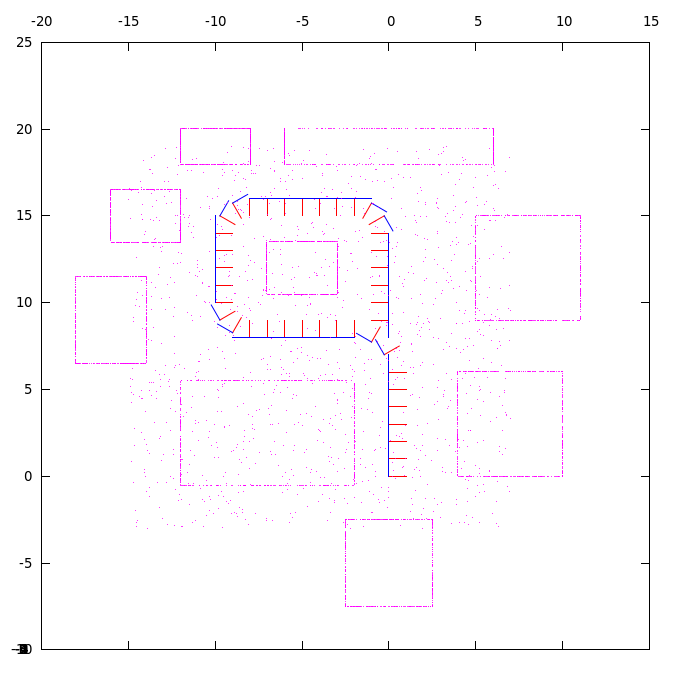
\includegraphics[width=0.45\linewidth]{images/createimage.png}}
\subfloat[Nuage recréé]{\label{fig:build}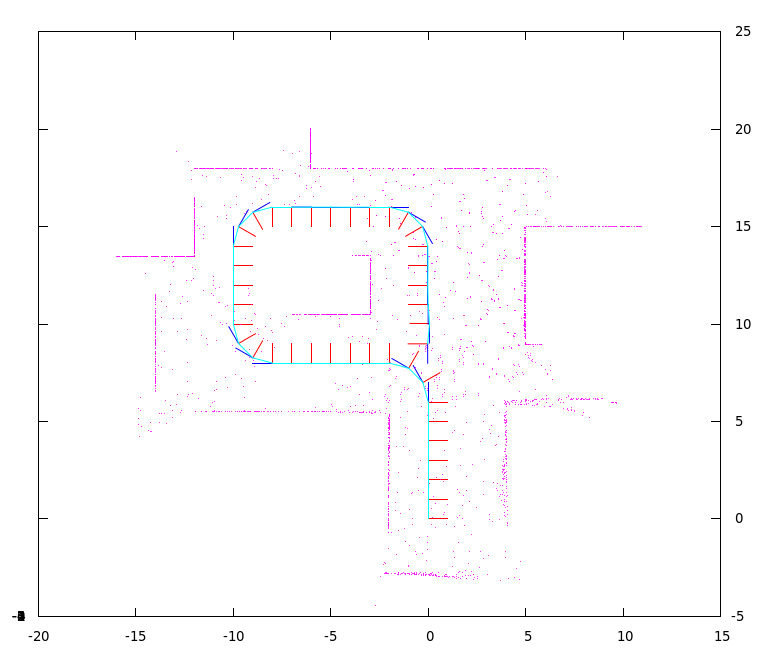
\includegraphics[width=0.45\linewidth]{images/buildfromvideo.png}}
\caption{L'image~\ref{fig:create} représente le nuage de points simulé ainsi que les différentes prises de vues, l'axe de la caméra ($\vec{z}$) est en bleu. Dans l'image~\ref{fig:build} on peut voir le résultat obtenu lors de la création du nuage à partir des images précédemment simulées.}
\end{center}
\end{figure}
\subsection{Travaux restants}

\subsubsection{Points importants}

Un certain nombre de points important reste cependant à explorer :
\begin{enumerate}
\item Vision : Afin de détecter les points en correspondance entre des images de types différents, nous avons besoin de tester d'autre descripteurs que SIFT, (SURF, MI, MSER, Ogre, \dots)
\item Ajustement de faisceaux : Dans le cas d'images provenant de caméras différentes et en prenant également en compte la dérive du facteur d'échelle
\item Temps réel : Établir une communication en temps réel entre les robots pour la fusion de carte (voir les travaux de R. \textsc{Aragues}~\cite{Aragues11PhD})
\item SoViN : Implémenter les fonctions manquantes dans SoViN puis le lier à ma bibliothèque 
\end{enumerate}

Ce projet étant étalé sur trois années, il reste donc deux ans et demi pour abordé en temps voulu les points précédents, je dois notamment mettre en place les idées suivantes :
\begin{enumerate}
\item Une surveillance dans un environnement dynamique et inconnu
\item Améliorer la localisation à l'aide de cartes topologiques ainsi qu'en utilisant les informations de position relatives entre les robots
\item Générer le suivi d'une cible à l'aide de plusieurs robots
\item Générer des déplacements en formation avec ou sans \emph{leader}
\end{enumerate}

\subsubsection{Grant}

Mettre un Grant ici \dag